%%%%%%%%%%%%%%%%%%%%%%%%%%%%%%%%%%%%%%%%%
% Formal Text-Rich Title Page
% LaTeX Template
% Version 1.0 (27/12/12)
%
% This template has been downloaded from:
% http://www.LaTeXTemplates.com
%
% Original author:
% Peter Wilson (herries.press@earthlink.net)
%
% License:
% CC BY-NC-SA 3.0 (http://creativecommons.org/licenses/by-nc-sa/3.0/)
%
% Instructions for using this template:
% This title page compiles as is. If you wish to include this title page in
% another document, you will need to copy everything before
% \begin{document} into the preamble of your document. The title page is
% then included using \titleGP within your document.
%
%%%%%%%%%%%%%%%%%%%%%%%%%%%%%%%%%%%%%%%%%

%----------------------------------------------------------------------------------------
%	PACKAGES AND OTHER DOCUMENT CONFIGURATIONS
%----------------------------------------------------------------------------------------

\documentclass{article}

\newcommand*{\plogo}{\fbox{$\mathcal{PL}$}} % Generic publisher logo

%----------------------------------------------------------------------------------------
%	TITLE PAGE
%----------------------------------------------------------------------------------------

\newcommand*{\titleGP}{\begingroup % Create the command for including the title page in the document
\centering % Center all text
\vspace*{\baselineskip} % White space at the top of the page

\rule{\textwidth}{1.6pt}\vspace*{-\baselineskip}\vspace*{2pt} % Thick horizontal line
\rule{\textwidth}{0.4pt}\\[\baselineskip] % Thin horizontal line

{\LARGE Empirical Study\\on\\[0.3\baselineskip] \ 10 IT Stocks in S\&P 500}\\[0.2\baselineskip] % Title

\rule{\textwidth}{0.4pt}\vspace*{-\baselineskip}\vspace{3.2pt} % Thin horizontal line
\rule{\textwidth}{1.6pt}\\[\baselineskip] % Thick horizontal line

\scshape % Small caps
Report for Statistical Language Programming\\[\baselineskip] % Tagline(s) or further description

\vspace*{2\baselineskip} % Whitespace between location/year and editors

Edited by \\[\baselineskip]
{\Large Fan,Song 578532\\Jinhua,Yang 578309\\ Wei,Zhang 578473\\Yue,Wang 578706\par} % Editor list


\vfill % Whitespace between editor names and publisher logo


{\large Humboldt-Universitaet zu Berlin}\par % Publisher

\endgroup}

%----------------------------------------------------------------------------------------
%	BLANK DOCUMENT
%----------------------------------------------------------------------------------------

\usepackage{fancyhdr}
\usepackage{indentfirst}
\usepackage{amsmath}
\usepackage{amssymb}
\usepackage{graphicx}
\usepackage[colorlinks,linkcolor=red]{hyperref}
\usepackage{listings}
\usepackage{natbib}
\lstset{language=R}
\lstset{breaklines}
\begin{document}
\pagestyle{empty} % Removes page numbers

\titleGP % This command includes the title page

    \newpage
    \pagestyle{fancy}\lhead{Report for Statistical Language Programming}\rhead{Fan,Song Jinhua,Yang\\Wei,Zhang Yue,Wang}
    \section{Introduction}

    \noindent Based on what we have learned in SLP courses and our interest in financial market, especially the behavior of stock prices, we collected share price data on 10 internet and software stocks, and conducted our empirical studies.
In our report, we write four programs, which can help us do statistical analysis of our data. We run panel regression, test for the CAPM theory, and estimate VaR of a price-weighted portfolio.\\
[\baselineskip]\indent Asset pricing theory and tine series study of the movement of stock prices are two major focus of finance. Investors use asset pricing theory to search for stocks which are underpriced and make profits by trading these stocks. There are also investors who believe in technical analysis, and they try to figure out the patterns in the movement of stock prices. These people often bet on the trends or momentum they discovered and trade according to their designed strategies.\\
[\baselineskip] \indent Stocks in the same industry may also have different performances, some stocks may have excess return compared to the market, while others are not. Assuming stocks in the same industry have the same reaction while market changes(same beta for all stocks), we apply panel regression to do this analysis. The basic model is pooled regression, which is to regress returns of all stocks on the market return and to see whether stocks this industry have excess return.\\
[\baselineskip] \indent Considering that the company¡¯s own characteristics may influence its stock performance, we also conduct the random- and fixed-effect model to see the effect.
 As the classical asset pricing theory, CAPM is always of great interest of scholars. If CAPM is true, and the stock prices are correctly priced, the estimated intercept of CAPM should not be significantly different from zero. Using our data, we can run CAPM regressions and use GRS test to see whether the intercepts of our regressions are significantly different from zero or not.\\
[\baselineskip] \indent Finally, we use DCC (Dynamic Conditional Correlation) model and calculated VaR for a price weighted portfolio constructed using these 10 stocks. And in order to test the robustness of our result, we apply DW and Engle's ARCH test to see whether the assumptions of our method are satisfied.

    \newpage
    \pagestyle{fancy}\lhead{Report for Statistical Language Programming}\rhead{Fan,Song Jinhua,Yang\\Wei,Zhang Yue,Wang}
    \section{Theory and Design}
    \subsection{Panel Data Analysis}
    \noindent We assume that the beta of all underlying stocks are the same, and the difference of returns are explained by individual effects, either fixed effects or random.\\
    [\baselineskip] \indent The basic panel data model \citep{baltagi2008econometric} is a pooled regression, which is:\\
    \begin{equation}\label{}
    R_{it}=\alpha_i+\beta R_{mt}+e_{it}\\
    \end{equation}
    In $(1)$, $R_{it}$ is the return of stock $i$ at time $t$;$\alpha_i$ is the idiosyncratic risk premium, $\beta$ is the part of risk premium that can be explained by the market factor, $R_{mt}$ is the market risk premium at time $t$, and $e_{it}$ is the residual.\\
    [\baselineskip] \indent As for the fixed effects model, in which the error term of pooled regression can be divided into two components, one of which is white noise and the other is the individual fixed-effects. The individual fixed-effect is represented by different intercept. This model can be expressed as follows:\\
    \begin{equation}\label{}
    R_{it}=\alpha_i+\beta R_{mt}+\mu_i+e_{it}\\
    \end{equation}
    Where
    \begin{equation}\label{}
    \varepsilon_{it}=\mu_i+e_{it},
    e_{it} \sim (0,\sigma^{2}_{e})\\
    \end{equation}
    $e_{it}$ is a random variable with expectation of 0 and homogeneous variance, and $\mu_{i}$ is the individual fixed-effects. And $E(u_i|R_{mt})\neq 0$.\\
    [\baselineskip] \indent When we using individual dummy variable to estimate the model, we simply use the OLS model:
    \begin{equation}\label{}
    R_{it}={com}_{1}+{com}_{2}+{com}_{3}+{com}_{4}+{com}_{5}+{com}_{6}+{com}_{7}+{com}_{8}+{com}_{9}+{com}_{10}+\beta R_{m}+e_{it}
    \end{equation}
    Where ${com}_{i}=1$ when the company is $i$ and $0$ otherwise and $e_{it} \sim (0,\sigma^{2}_{e})$.\\
    The random effect model is:\\
    \begin{equation}\label{}
    R_{it}=\alpha_i+\beta R_{mt}+\mu_i+e_{it}\\
    \end{equation}
    Where
    \begin{equation}\label{}
    \varepsilon_{it}=\mu_i+e_{it},
    e_{it} \sim (0,\sigma^{2}_{e})\\
    \end{equation}
    In this mode we assume $mu_{i}$ is a random variable with expectations conditional on $R_{it}$ equal to zero. Since the whole error term $\epsilon_{it}$ violates the assumption of OLS, we use GLS to estimate the random effect model.\\

    \subsection{Test of CAPM}
    \noindent However, in the test of CAPM, we drop the assumption that all stocks have the same beta, and assume they differ from each other. Firstly, we used the seemingly unrelated regression model to estimate $\beta_{i}$ for each company. The model \citep{sharpe1964capital, sharpe1970portfolio}can be expressed as follows:\\
    \begin{equation}\label{}
    Z_{it}=\alpha_{i}+\beta_{i}Z_{mt}+\epsilon_{it}
    \end{equation}
    Where $Z_{it}$ is the excess return of the stock of company $i$ at time $t$, which can be calculated as follows:\\
    \begin{equation}\label{}
    Z_{it}=E(R_{i})-R_{f}
    \end{equation}
    At last, we use GRS test to test the null hypothesis that all of the intercepts are jointly equal to zero, i.e.:\\
    \begin{equation}\label{}
    H_{0}:\alpha_{1}=\alpha_{2}=...=\alpha_{10}=0
    \end{equation}
    GRS test \citep{gibbons1989test} statistic:\\
    \begin{equation}\label{}
    \frac{T(T-N-1)}{N(T-2)}\cdot \frac{\hat{\alpha}'\cdot \Sigma^{-1}\cdot \hat{\alpha}}{1+S^2_{m}}\overset{H_{0}}\sim F_{N,T-N-1}
    \end{equation}
    Where $S_{m}$ is the sharp ratio, which can be calculated as follows:\\
    \begin{equation}\label{}
    S_{m}=\frac{E(R_{m}-R_{f})}{\sigma_{m}}
    \end{equation}

    \subsection{Estimation of Portfolio VaR}
    \noindent VaR can be computed according to the following formula:\\
    \begin{equation}\label{}
    VaR=W_{0}\cdot(Z\cdot\sigma+\mu)
    \end{equation}
    Where $W_{0}$ is the initial wealth, $Z$ is the underlying confidence level, $\sigma$ and $\mu$ are the variance and mean of related asset return respectively.\\
    [\baselineskip] \indent Once we know the variance of the investment asset and its mean, we can easily compute it VaR. In our analysis, we constructed a price-weighted portfolio using the 10 chosen stocks, which means the weight of every stock is proportional to its initial share price. To state differently, in our portfolio, we long one share of every selected stock.\\
    [\baselineskip] \indent We assume that every stock has autocorrelation and ARCH effect, the empirical variance of portfolio return was not proper to be used to compute VaR, therefore, estimating the variance-covariance matrix is necessary. There are two alternative ways to compute the variance and covariance matrix. The first option is multivariate GARCH models, it can capture volatility clustering and correlation of asset returns. However, multivariate GARCH model suffers from huge parameter spaces. And traditional correlation models have problem with higher dimensional systems. As a substitute, we used dynamic conditional correlation (DCC) models, which is the trade-off between model feasibility and flexibility. The explicit model is as follows:\\
    \begin{eqnarray}\label{}
    \begin{split}
    h_{t}&=\alpha+A\epsilon^{2}_{t-1}+Bh_{t-1}\\
    \epsilon_{i,t}&=h^{1/2}z_{i,t}\\
    z_{t}&\sim ID(0,P_{t})
    \end{split}
    \end{eqnarray}
    DCC model \citep{engle2002dynamic} is as follows:\\
    \begin{eqnarray}\label{}
    \begin{split}
    P_{t}&=(Q_{T}\bigodot I_{N})^{-1/2}Q_{T}(Q_{T}\bigodot I_{N})^{-1/2}\\
    Q_{T}&=(1-\alpha-\beta)Q+\alpha Z_{t-1}Z'_{t-1}+\beta Q_{t-1}\\
    \alpha+\beta &<1\\
    \alpha ,\beta &>0
    \end{split}
    \end{eqnarray}
    Where $Q$ is a sample covariance matrix of $Z_{t}$.\\
    [\baselineskip] \indent In the end, in order to test whether our time series fulfill the assumption that they have autocorrelation and ARCH effect, we simply used the build-in function of DW-test \citep{durbin1950testing,durbin1951testing} and Engle's ARCH test \citep{engle1982autoregressive}.\\
    \newpage
    \pagestyle{fancy}\lhead{Report for Statistical Language Programming}\rhead{Fan,Song Jinhua,Yang\\Wei,Zhang Yue,Wang}
    \section{Implementation}
    \subsection{Data Description}
    \noindent Core part of our code:\\
    \begin{lstlisting}[language=R,numbers=left, numberstyle=\normalsize]
    summary(Paneldata$Ri)
    summary(Paneldata$Rm)
    stargazer(Paneldata)
    p = ggplot(Paneldata, aes(x = Rm,y = Ri,colours = factor(company)))
    p + geom_point(aes(colour = factor(company))) + stat_smooth()
    p = ggplot(Paneldata, aes(x = Ri))
    p + geom_histogram(aes(fill = factor(company), y = ..density..), alpha = 0.3, colour = "blue") +  stat_density(geom = "line", position = "identity", size = 1.5, aes(colour = factor(company))) + facet_wrap(~company, ncol = 1)
    plotmeans(Ri ~ company, main = "Heterogeineity across companies", data = Paneldata)
    plotmeans(Ri ~ date, n.label = FALSE, main = "Heterogeneity across time", data = Paneldata)
    \end{lstlisting}

    \noindent Firstly we focus on the descriptive analysis of the panel data. We use `summary()' function in line 1 and 2 and to conclude the descriptive analysis(mean, min, max and other statistics of our data) and use `stargazer' package to make LaTex table as stated in line 3.\\


    \subsection{Panel Analysis}
    \subsubsection{Pooled regression}
    \noindent Core part of our code:\\
    \begin{lstlisting}[language=R,numbers=left, numberstyle=\normalsize]
    pooling=plm(Ri~Rm,data=Paneldata,index=c("company","date"),model="pooling")
    plot(Ri ~ Rm, data = Paneldata, main = "relationship between market return and stock return",  xlab = "market return", ylab = "stock return")
    model = lm(Ri ~ Rm)
    abline(model, col = "red")

    \end{lstlisting}
    In line 1 we use the `plm' command to do the pooled regression. Then we use the `plot' commad to plot out the distribution of the residuals of this regression and use `qqnorm' command in line 6 to analyze whether the normality assumption is satisfied in this model.\\

    \subsubsection{Fixed and Random Effect Model}
    \noindent Core part of our code:\\
    \begin{lstlisting}[language=R,numbers=left, numberstyle=\normalsize]
    xyplot(Ri ~ Rm | com, data = Paneldata, panel = function(x, y) {
    panel.xyplot(x, y)
    panel.abline(h = median(y), lty = 2, col = "gray")
    panel.lmline(x, y, col = "red")
    }, xlab = "market return", ylab = "stock return", main = "relationship between market return and stock return")
    fixed.dum=lm(Ri~Rm+factor(com)-1,data=Paneldata)
    yhat=fixed.dum$fitted.values
    scatterplot(yhat ~ Rm | Paneldata$company, boxplots = FALSE, xlab = "Market price", ylab = "yhat", legend.plot = FALSE,
    main="Fixed effects regression vs. Pooling Regression",
    smooth = FALSE)
    abline(lm(Ri ~ Rm), lwd = 3, col = "Dark Blue")
    fixed=plm(Ri~Rm,data=Paneldata,index=c("company","date"),model="within")
    test_fixed = pFtest(fixed, pooling)
    random=plm(Ri~Rm,data=Paneldata,index=c("company","date"),model="random")
    phtest(fixed,random)
    \end{lstlisting}
    \indent First of all, we use `xyplot' command in line 1 to analyze graphically whether it is obvious that there are individual fixed effects.\\
    [\baselineskip]\indent Then we use `lm' command in line 4 to do least squared dummy variable regression. And then from line 5, we analyze graphically the linear regression line for each company and the overall regression using command `scatterplot'.\\
    [\baselineskip]\indent And we use `plm' command to estimate the fixed-effect model and random-effect model by setting the `model' variable equal to `within' and `random'. Then make comparison between pooled model and fixed model by `pFtest'(F-test), fixed-effect model and random-effect model by `phtest'(Hausemantest) in line 14 and 16 separately.\\

    \subsection{Test of CAPM}
    \subsubsection{Seemingly Unrelated Regression for CAPM}
    \noindent Core part of our code:\\
    \begin{lstlisting}[language=R,numbers=left, numberstyle=\normalsize]
Google = Capm$Google
Ebay = Capm$Ebay
Facebook = Capm$Facebook
Yahoo = Capm$Yahoo
WU = Capm$WU
Verisign = Capm$Verisign
Netflix = Capm$netflix
TSS = Capm$TSS
FNI = Capm$FNI
ADP = Capm$ADP
amer = Capm$amer
xyplot(aser ~ amer | com, data = Paneldata, panel = function(x, y) {
panel.xyplot(x, y)
panel.abline(h = median(y), lty = 2, col = "gray")
panel.lmline(x, y, col = "red")
}, xlab = "average excess market return", ylab = "average excess stock return", xlim = c(0, 2), ylim = c(0,5), main = "Excess market return and excess stock return")

eq1=Google~amer
eq2=Ebay~amer
eq3=Facebook~amer
eq4=Yahoo~amer
eq5=WU~amer
eq6=Verisign~amer
eq8=TSS~amer
eq9=FNI~amer
eq10=ADP~amer
system=list(eq1=eq1,eq2=eq2,eq3=eq3,eq4=eq4,eq5=eq5,eq6=eq6,eq8=eq8,eq9=eq9,eq10=eq10)
sur=systemfit(system,method="SUR",data=Capm)
summary(sur)

    \end{lstlisting}
    From line 1 to line 10, we name the average excess stock return of different companies with the company initials. Line 11 we denote the average market excess return with `amer'.\\
    [\baselineskip]\indent In line 12, we use `xyplot' command to plot out the scatterplot graph of the relationship between average excess stock return and average market return for the 10 companies and add the regression lines to see whether the intercepts of the regression lines are close to 0.\\
    [\baselineskip]\indent From line 13 to line 26, we define the 9 regression models of the excess return of stocks for each companies on the average excess return of market portfolio. And in line 27, we use `list' command to define the system of equations and then use `systemfit' command to estimate the SUR model.\\


    \subsubsection{GRS test for CAPM}
    \noindent Core part of our code:\\
    \begin{lstlisting}[language=R,numbers=left, numberstyle=\normalsize]
Capm1 = read.csv("Capm1.csv")
sur1 = matrix(sur$coefficients, nrow = 2, ncol = 9)
alphas = sur1[1, ]
sig.hat=sur$residCov
sample.sr = function(x) {mu = mean(x);sg = sd(x);return(mu / sg)}
amer=Capm1$amer
mkt.sr=sample.sr(amer)
GRS.stat=t(alphas)%*%solve(sig.hat,(alphas))/(1+mkt.sr^2)
T=52
N=9
F.stat=T*(T-N-1)*GRS.stat/(N*(T-2))
p.val=pf(F.stat,N,T-N-1,0,lower.tail = F)
    \end{lstlisting}
    Since there is no GRS test package in R yet, we use function command to calculate the statistics and calculate the p-value. Firstly, in line 3 and line 4 we define alphas as the intercepts and `sig.hat' as the residual covariance matrix from the SUR regression we run previously. After that, we define a function to calculate the sample sharp ratio as stated in line 5. Then we calculate the market sharp ratio use this function in line 7. Finally we define the GRS statistics based on its formula as in line 8 and calculate the corresponding F statistics and the p-value.\\

    \subsection{Estimation of Portfolio VaR}
    \subsubsection{VaR Estimation}
    \noindent Core part of our code:\\
    \begin{lstlisting}[language=R,numbers=left, numberstyle=\normalsize]
return = log(price[2, ]/price[1, ])
for (j in 2:(T - 1)) {
return[j, ] = log(price[j + 1, ]/price[j, ])
}
for (j in 1:(T - t)) {ts = return[j:(j + t - 1), ]
for (i in 1:n) {residual[, i] = matrix(residuals(arma(ts[, i], order = c(1, 0))))}

for (i in 1:10) {coef[i, ] = matrix(coef(garch(residual[, i], order = c(1, 1), series = NULL)))}

# DCC-GARCH model estimation
a = coef[, 1]
A = diag(coef[, 2])
B = diag(coef[, 3])
dcc.para = c(0.01, 0.97)
results = dcc.estimation(inia = a, iniA = A, iniB = B, ini.dcc = dcc.para, dvar = residual, model =       "diagonal")
h = results$h
dcc = results$DCC
v = sqrt(diag(h[t - 1, ]))
R = matrix(data = dcc[1, ], nrow = n, ncol = n)
H = v %*% R %*% v

VaR95[j, ] = sqrt(t(W) %*% H %*% W) * alpha95 * value[j]
VaR99[j, ] = sqrt(t(W) %*% H %*% W) * alpha99 * value[j]}
PL = value[(t + 1):T, ] - value[t:(T - 1), ]
matplot(c(1:(T - t)), bt[, 1:3], type = "l", xlab = "time", ylab = "P&L", xaxt = "n")
colnames(bt) = c("PL", "95%VaR", "99%VaR")
legend("topright", colnames(bt)[-1], lwd = 1, col = 2:3, cex = 0.75)
title("Portfolio P&L and estimated VaR")
axis(1, at = c(1:(T - t)), las = 0)
    \end{lstlisting}
    In order to get the daily log return of each stock, we use line 1 to initialize the return variable and use `for' command in line 2 to apply the log return formula for every row regardless the columns, thus we can get the daily return for every stock. In line 3, when we fix the length of our rolling screen `t', the number of VaR we estimate for our portfolio will be T-t. Thus we run j from 1 to T-t, to get every estimation of VaR. And for every VaR, we use the stick returns from j to j+t-1 of each stock, thus each stock has t observations for parameter estimation. In line 4, in order to get arma residual for every stock in each rolling screen, we use `for' command running for each stock and use `arma' function with order (1,0) with our model being AR(1).\\
    [\baselineskip]\indent From the above process, we get n*3 coefficients in total, which is the input for DCC model. Through DCC model in line 11, we get the variance as in line 12, correlation coefficients as in line 13. Use the variance of the last day, and compute them with the correlation coefficients and we can get variance-covariance matrix. Together with the weights of portfolios, we finally obtain the variance of our portfolio, which is the critical input for our estimation of VaR. This whole process is repeated for T-t times, where T is the number of days, t is the number of days in the chosen rolling screen.\\
    [\baselineskip]\indent Using the estimated coefficient from initial GARCH model, residuals from AR(1) model, together with other initial parameters we use `dcc.estimation' function and the variance and correlation coefficient can be estimated. `v' in line 18 is the square root of variance, `R' in line 19 is the correlation coefficient, then by line 20 we can get the variance of our price weighted portfolio. In line 22 and 23 the 95\% and 99\% VaRs are estimated.\\
    [\baselineskip]\indent In line 24, we computed the daily profit and loss of each stock. `Matplot' function in line 25 is a function for matrix plot, here we use this to plot 3 lines (P\&L,VaR95, and VaR99) together at once. And in line 29, we use `axis' function to create new format for x-axis, and `at' indicates the tic marks we drawn are related to the number of rolling screen, which is also the number of VaRs we estimate.\\

    \subsubsection{DCC Model Assumption}
    \noindent Core part of our code:\\
    \begin{lstlisting}[language=R,numbers=left, numberstyle=\normalsize]
for (i in 1:10) {
dw = dwtest(return[2:247, i] ~ return[1:246, i] pvalue_dwtest[, i] = dw$p.valuedw_stat[, i] =     dw$statistic
}
pvalue_dwtest = as.data.frame(pvalue_dwtest)
dw_stat = as.data.frame(dw_stat)

return1 = as.list(return)
archtest = lapply(return1, ArchTest, lags = 8, demean = TRUE)
a = as.data.frame(matrix((unlist(archtest)), c(5, 10)))
LM_test_ARCH = rbind(a[1, ], a[3, ])
    \end{lstlisting}

   \noindent To test the two assumptions for DCC model, we used `lmtest' and `FintTS' package. From line 1 to 3, we conducted a DW test, and in line 8 we conducted the Engle's ARCH test for all of our time series. In line 1, we used `for' command to repeat the DW test for our 10 selected stocks, can get the DW statistics and corresponding p value. In line 8, we use `lapply' function to apply `ArchTest' to all columns and obtained the corresponding statistics and p values.\\

    \newpage
    \pagestyle{fancy}\lhead{Report for Statistical Language Programming}\rhead{Fan,Song Jinhua,Yang\\Wei,Zhang Yue,Wang}
    \section{Empirical Study/Testing}
    \subsection{Data Input}
    \noindent We collect daily stock price and S\&P 500 index from
    \url{http://finance.yahoo.com/} for the following 10 stocks:\\
    \begin{center}
    \begin{table}[!htbp] \centering 
 
	\label{}  
	\begin{tabular}{@{\extracolsep{5pt}}l|ccccc} 
		\hline 
		\hline \\[-1.8ex] Name of the company
		& \multicolumn{1}{c}{Ticker
		}  \\ 
		\hline \\[-1.8ex] 
		Google & GOOGL \\ 
		Ebay & EBAY \\ 
		Facebook & FB\\ 
		Yahoo & YHOO \\ 
		Wester Union & WU\\ 
		Verisign Inc & VRSN \\ 
		Netflix Inc. & NFLX \\ 
		Total System Service &TSS \\ 
		Fidelity National Information Services & FIS \\ 
		Automatic Data Processing & ADP \\ 
		\hline\hline 
	\end{tabular} 
	\caption{Stock List}
\end{table}
    \end{center}
    And we use the Treasury bill rate of US as the risk free rate, which is available at\\ \url{https://www.treasury.gov/resource-center/data-chart-center/interes-trates/Pages/TextView.aspx?data=yield}.\\
    [\baselineskip] \indent The time period for these data is 01/05/2015-25/04/2016. For panel analysis we use weekly return of these stocks, for test of CAPM we use three-month return of these stocks, for the estimation of VaR we use daily return of these stocks.//
    The raw data we obtain directly from this resources are prices (daily or weekly), and we need to pre-process them by applying the function\\
    \begin{center}
    $R_{t+1}=\ln{\frac{P_{t+1}}{P_{t}}}$ \\
    \end{center}
    to get the return of individual stock and the market.

    \subsection{Pooled Regression Model}
    \begin{itemize}
    \item \textbf{Function}
    \end{itemize}
    \begin{lstlisting}[language=R,numbers=left, numberstyle=\normalsize]
    pooling = plm(Ri ~ Rm, data = Paneldata, index = c("company", "date"), model = "pooling")
    \end{lstlisting}
    \begin{itemize}
    \item \textbf{Input Description}
    \end{itemize}
    \noindent Use the data source as stated above, in which Ri is the individual stock return while Rm is the market return. This is panel data, in which `company' is the `individual' and `date' stands for `time'. Hence the `index' in the function is to tell R which is individual and which is time.\\

    Besides, we denote the ten companies as the number 1 to 10. For each company there are 52 time periods and corresponding $R_{i}$. There are also 52 periods for $R_{m}$ and for each company $R_{m}$ is the same.\\

    For pooled regression model, we pool the data together and do OLS.\\


    \begin{itemize}
    \item \textbf{Expected Output}
    \end{itemize}
    We expect a positive relation between market portfolio return and the stock return overall.\\


    \begin{itemize}
    \item \textbf{Actual Output}
    \end{itemize}
    \begin{center}
\begin{table}[!htbp] 
	\centering 
	\begin{tabular}{@{\extracolsep{0.2pt}}l|c} 
		\hline 
		\hline \\[-2.0ex] 
		& \multicolumn{1}{c}{\textit{Dependent variable:}} \\ 
	
		\\[-2.0ex] & Ri \\ 
		\hline \\[-1.8ex] 
		
		Rm & 1.235$^{***}$ \\ 
		& (0.071) \\ 
	    \\[-2.0ex]
		Constant & 0.003$^{**}$ \\ 
		& (0.001) \\ 
		
		\hline \\[-1.8ex] 
		Observations & 520 \\ 
		R$^{2}$ & 0.368 \\ 
		Adjusted R$^{2}$ & 0.366 \\ 
		F Statistic & 301.162$^{***}$  \\ 
		\hline 
		\hline 
		
	\end{tabular} 
	\caption{Pooled Regression Results} 
\end{table} 

    \end{center}

    \begin{itemize}
    \item \textbf{Comments}
    \end{itemize}
    \noindent The market portfolio return and stock return are actually positive correlated. And the coefficient is significant under the significance level of 1\%. According to the F statistic, the model is significant.\\

    \subsection{Fixed Effect Regression Model}
    \begin{itemize}
    \item \textbf{Function}
    \end{itemize}
    \begin{lstlisting}[language=R,numbers=left, numberstyle=\normalsize]
fixed = plm(Ri ~ Rm, data = Paneldata, index = c("company", "date"), model = "within")
    \end{lstlisting}
    \begin{itemize}
    \item \textbf{Input Description}
    \end{itemize}
    \noindent We employ the panel data as we stated in the pooled regression model. Including fixed effects across companies, we use within estimator approach, which is that we subtract Ri, Rm and also the error term with their corresponding average, and then do the OLS regression. Here for the `model' part we input 'within'.\\

    \begin{itemize}
    \item \textbf{Expected Output}
    \end{itemize}
    \noindent According to graphical analysis, we figured that the fixed effects of different companies is not very obvious.\\

    \begin{itemize}
    \item \textbf{Actual Output}
    \end{itemize}
    \begin{center}
\begin{table}[ht] 
	\centering 
	 
	\label{} 
	\begin{tabular}{@{\extracolsep{5pt}}l|c} 
		\hline 
		\hline \\[-2.0ex] 
		& \multicolumn{1}{c}{\textit{Dependent variable:}} \\ 
		
		\\[-2.0ex] & Ri \\ 
		\hline \\[-1.8ex] 
		Rm & 1.235$^{***}$ \\ 
		& (0.071) \\ 
		
		\hline \\[-1.8ex] 
		Observations & 520 \\ 
		R$^{2}$ & 0.370 \\ 
		Adjusted R$^{2}$ & 0.362 \\ 
		F Statistic & 298.774$^{***}$  \\ 
		\hline 
		\hline 
		
	\end{tabular} 
	\caption{Fixed Effects Regression Using plm}
\end{table} 
    \end{center}

    \begin{itemize}
    \item \textbf{Comments}
    \end{itemize}
    \noindent The coefficient value and the variance of the coefficient are the same with pooled regression model. It is likely that there is no significant difference between fixed effects model and pooled regression model.\\


    \subsection{Testing for Fixed Effects}
    \begin{itemize}
    \item \textbf{Function}
    \end{itemize}
    \begin{lstlisting}[language=R,numbers=left, numberstyle=\normalsize]
test_fixed = pFtest(fixed, pool)
    \end{lstlisting}
    \begin{itemize}
    \item \textbf{Input Description}
    \end{itemize}
    \noindent After finishing the regressions of fixed effects model and pooled model, we use the F-test to test whether the fixed effects across companies are significant. Note that this step is based on the fact that we have already finished the two regressions. Then we use the denoted results, here `fixed' and `pool', from the two regressions to do the F-test.\\


    \begin{itemize}
    \item \textbf{Expected Output}
    \end{itemize}
    \noindent As stated in the last part, we expect no significant fixed effects between companies.\\

    \begin{itemize}
    \item \textbf{Actual Output}
    \end{itemize}
    F test for individual effects\\
    data:  Ri\~Rm\\
    F = 0.54364, df1 = 9, df2 = 509, p-value = 0.8427\\
    Alternative hypothesis: significant effects.\\

    \begin{itemize}
    \item \textbf{Comments}
    \end{itemize}
    p-value is much larger than 5\%, which means that there is no evidence proving that the Fixed Effects Model is better than Pooled Regression Model.\\

    \subsection{Random Effect Regression Model}
    \begin{itemize}
    \item \textbf{Function}
    \end{itemize}
    \begin{lstlisting}[language=R,numbers=left, numberstyle=\normalsize]
random = plm(Ri ~ Rm, data = Paneldata, index = c("company", "date"), model = "random")
    \end{lstlisting}
    \begin{itemize}
    \item \textbf{Input Description}
    \end{itemize}
    Again we use the panel data described in pooled regression model. Here for the `model' part we input `random'. The underlying approach used in this function is actually GLS estimation owing to the structure of the error term in random effects model.\\

    \begin{itemize}
    \item \textbf{Expected Output}
    \end{itemize}
    Since we expect that the effects is related to the regressor, that is, the important assumption for random effects model,$E(u_i|R_{mt})\neq 0$, is not satisfied. Therefore we expect random effects model should generate the same outcome as pooled effects model.\\

    \begin{itemize}
    \item \textbf{Actual Output}
    \end{itemize}
    \begin{center}
\begin{table}[ht] \centering 
		
	
		\begin{tabular}{@{\extracolsep{5pt}}l|c} 
			\hline 
			\hline \\[-2.0ex] 
			& \multicolumn{1}{c}{\textit{Dependent variable:}} \\ 
			 
			& Ri \\ 
			\hline \\[-1.8ex] 
			Rm & 1.235$^{***}$ \\ 
			& (0.071) \\ 
			\\[-2.0ex]
			Constant & 0.003$^{***}$ \\ 
			& (0.001) \\ 
			
			\hline \\[-1.8ex] 
			Observations & 520 \\ 
			R$^{2}$ & 0.366 \\ 
			Adjusted R$^{2}$ & 0.365 \\ 
			F Statistic & 299.657$^{***}$  \\ 
			\hline 
			\hline 
			
		\end{tabular}
		\caption{Random Effects Regression}  
	\end{table} 
    \end{center}
    \begin{itemize}
    \item \textbf{Comments}
    \end{itemize}
    Just as we expected, the random effects regression result is almost the same with pooled regression except for a slightly lower R-squared and F-statistic.\\


    \subsection{Testing for the Fixed Effects Model and Random Effects Model}
    \begin{itemize}
    \item \textbf{Function}
    \end{itemize}
    \begin{lstlisting}[language=R,numbers=left, numberstyle=\normalsize]
phtest(fixed, random)
    \end{lstlisting}
    \begin{itemize}
    \item \textbf{Input Description}
    \end{itemize}
    After finishing both fixed effects model regression and random effects model regression, we denote the two models as `fixed' and `random'. And then use Hausman test to test whether within estimator or GLS estimator is consistent.\\

    \begin{itemize}
    \item \textbf{Expected Output}
    \end{itemize}
    We expect there is random effects model is inconsistent, that is, we expect that we would reject the null hypothesis.\\

    \begin{itemize}
    \item \textbf{Actual Output}
    \end{itemize}
    Hausman Test\\
    data:  $Ri \sim Rm$\\
    chisq = 4.7193e-25, df = 1, p-value = 1\\
    alternative hypothesis: one model is inconsistent\\


    \begin{itemize}
    \item \textbf{Comments}
    \end{itemize}
    We cannot reject null hypothesis, which is that the preferred model is random effects. Thus comparing with Fixed Effects Model, Random Effects Model is better.\\

    \subsection{Comparison of Random Effects Model and Pooled Regression Model}
    \begin{itemize}
    \item \textbf{Function}
    \end{itemize}
    \begin{lstlisting}[language=R,numbers=left, numberstyle=\normalsize]
    plmtest(pooling)
    \end{lstlisting}
    \begin{itemize}
    \item \textbf{Input Description}
    \end{itemize}
    Use the result of the random effects model and pooled regression model.\\

    \begin{itemize}
    \item \textbf{Expected Output}
    \end{itemize}
    We expect that we cannot reject the null hypothesis since we expect that the assumption $E(u_i|R_{mt})\neq 0$ may not be satisfied.\\

    \begin{itemize}
    \item \textbf{Actual Output}
    \end{itemize}
    Lagrange Multiplier Test - (Honda)\\
    data:  Ri\~Rm\\
    normal = -1.14, p-value = 0.2543\\
    Alternative hypothesis: significant effects\\


    \begin{itemize}
    \item \textbf{Comments}
    \end{itemize}
    P-value is too high. We cannot reject the null hypothesis. It is better to use Pooled Regression Model.\\

    \subsection{CAPM testing-SUR and GRS test}
    \begin{itemize}
    \item \textbf{Function}
    \end{itemize}
    \begin{lstlisting}[language=R,numbers=left, numberstyle=\normalsize]
sur=systemfit(system,method="SUR",data=Capm)
sur1=matrix(sur$coefficients,nrow=2,ncol=9)
alphas=sur1[1,]
sig.hat=sur$residCov
sample.sr = function(x) {mu = mean(x);sg = sd(x);return(mu / sg)}
amer=Capm1$amer
mkt.sr=sample.sr(amer)
GRS.stat=t(alphas)%*%solve(sig.hat,(alphas))/(1+mkt.sr^2)
T=nrow(Capm1)
N=ncol(Capm1)-3
F.stat=T*(T-N-1)*GRS.stat/(N*(T-2))
p.val=pf(F.stat,N,T-N-1,0,lower.tail = F)

    \end{lstlisting}
    \begin{itemize}
    \item \textbf{Input Description}
    \end{itemize}
    \noindent We use the 3-months Treasury bill yield as the risk-free interest rate and calculate out the averaged market excess return and excess stock return (both for 3 months). We put the adjusted data to a file `Capm', and we execute the SUR and GRS test.\\

    First we should take out all the intercepts of the seemly uncorrelated regressions, which is done by the 2nd and 3rd lines of the functions. If the input of the functions is wrong, then the $\alpha$ we get would be wrong.\\

    Then we should get the variance-covariance matrix of the error terms of the SUR, which is done by the 4th line. And from 5th to 7th lines we get the sample market sharp ratio. The function of the 5th line is merely the sharp ratio function. And in the 6th and 7th lines we insert the averaged market excess return into this function and calculate the sample market sharp ratio. If the function is wrong or what we input is not averaged market excess return, then the result we get would be wrong.\\
    The 8th line is to calculate the GRS statistic. We input the alpha, variance-covariance matrix as well as the sample market sharp ratio into this function and get the GRS statistic. And then based on this, the 9th line get the F statistic and thus the p-value. Any incorrect input for these functions would lead to a wrong output (econometrically speaking).\\


    \begin{itemize}
    \item \textbf{Expected Output}
    \end{itemize}
    We expect that we can reject the null hypothesis that all of the intercepts of the SUR are jointly zero\\


    \begin{itemize}
    \item \textbf{Actual Output}
    \end{itemize}
    P-value= 0.002696034\\

    \begin{itemize}
    \item \textbf{Comments}
    \end{itemize}
    We can reject the null hypothesis that the intercepts are $0$. However, this does not necessarily mean that CAPM is a wrong model.\\

    \subsection{Estimation of VaR}
    \begin{itemize}
    \item \textbf{Input Description}
    \end{itemize}
    In this sub-program, raw data of daily prices can be directly used as the input. After computing the daily return, we constructed a price weighted portfolio, and then use the return of this portfolio to calculated our 95\% and 99\% VaR. For a normal case input, we choose rolling screen size t=200.\\

    \begin{itemize}
    \item \textbf{Expected Output}
    \end{itemize}
    Through our programming, we expect to compute T-t, which is 248-200=48 95\% and 48 99\%VaRs, they should be parallel to each other and the 99\% VaR has larger absolute value than the 95\% VaR.\\

    \begin{itemize}
    \item \textbf{Actual Output}
    \end{itemize}
    \begin{center}
    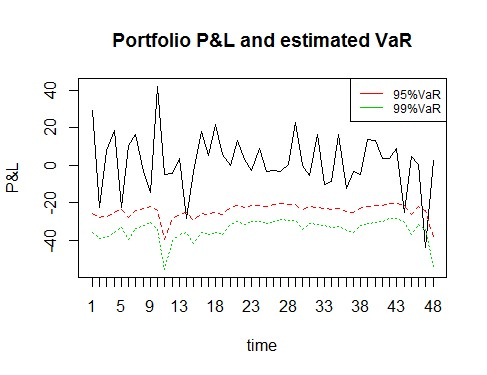
\includegraphics[scale=1]{5.jpg}%µÚÎåÕÅͼ
    \end{center}
    \begin{itemize}
    \item \textbf{Comments}
    \end{itemize}
    It is clear that given related data, our program can effectively calculate the 95\% and 99\% VaR of price weighted portfolio constructed using selected stocks. There are only 3 outliers given 95\%VaR estimated, and only 1 outlier given 99\%VaR estimated. In the programming, we use DCC GARCH model, which is a generalization of the CCC GARCH model and allows the correlation matrix to depend on time. The DCC GARCH model has clear computational advantages in that the number of parameters to be estimated in the correlation process is independent of the number of series to be correlated. Thus potentially very large correlation matrices can be estimated.\\

    \begin{itemize}
    \item \textbf{Test for Extreme Case\:t=247}
    \end{itemize}
    Expected output: 3 dots\\
    Actual output: no output.\\
    Reason: Due to limitation of `matrix plot function', it cannot produce any output graph when there is only one row of observation.\\

    \begin{itemize}
    \item \textbf{Test for Special Case\:t=246}
    \end{itemize}
    Expected output: 3 straight lines. When t=246, there are 2 estimations for each portfolio VaR, and with two dots, a straight line can be defined.\\
    Actual output: good output.\\
    \begin{center}
    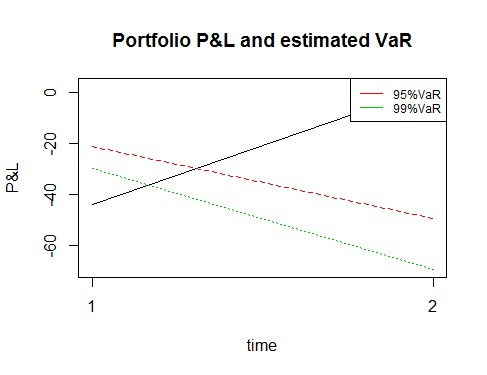
\includegraphics[scale=1]{6.jpg}%µÚÁùÕÅͼ
    \end{center}
    Comments: matrix plot can be implemented with 2 rows.\\


    \subsection{DCC Assumptions Test}
    \begin{itemize}
    \item \textbf{Input Description}
    \end{itemize}
    For this sub-program, raw data of daily stock prices can also be directly used as input.\\
    \begin{itemize}
    \item \textbf{Expected Output}
    \end{itemize}
    Since our calculation of VaR using DCC model is based on the critical assumptions that the time series have autocorrelation and ARCH effect, we expect the test results to be significantly different from zero, with P-values being small enough (at least <10\%). Otherwise, our calculation result would not make sense.\\
    \begin{itemize}
    \item \textbf{Actual Output}
    \end{itemize}
    \begin{center}
\begin{table}[!htbp] \centering 
	
	\label{} 
	\begin{tabular}{@{\extracolsep{5pt}}l|ccccc} 
	    \hline 
		\hline \\[-1.8ex] 
		& \multicolumn{1}{c}{GOOGL} & \multicolumn{1}{c}{EBAY} & \multicolumn{1}{c}{FB} & \multicolumn{1}{c}{YHOO} & \multicolumn{1}{c}{WU} \\ 
		\hline \\[-1.8ex] 
		dw\_stat & 1.98 & 1.99 & 1.99 & 2.00 & 1.99 
		\\ 
		p\_value & 0.44 & 0.47 & 0.48 & 0.52 & 0.49 
		\\ 
		\hline\hline 
	\end{tabular} 
	\\[2.8ex]
	\begin{tabular}{@{\extracolsep{5pt}}l|ccccc} 
		\hline 
		\hline \\[-1.8ex] 
		& \multicolumn{1}{c}{VRSN} & \multicolumn{1}{c}{NFLX} & \multicolumn{1}{c}{TSS} & \multicolumn{1}{c}{FIS} & \multicolumn{1}{c}{ADP} \\ 
		\hline \\[-1.8ex] 
		dw\_stat & 1.98 & 1.99 & 1.98 & 2.02 & 1.99
		\\ 
		p\_value & 0.44 & 0.47 & 0.46 & 0.57 & 0.49
		\\ 
		\hline\hline  
	\end{tabular} 
	\caption{DW-Test} 
\end{table}
    \end{center}
    \begin{center}
\begin{table}[!htbp] \centering 
	
	\label{} 
	\begin{tabular}{@{\extracolsep{5pt}}l|ccccc} 
		\hline 
		\hline \\[-1.8ex] 
		& \multicolumn{1}{c}{GOOGL} & \multicolumn{1}{c}{EBAY} & \multicolumn{1}{c}{FB} & \multicolumn{1}{c}{YHOO} & \multicolumn{1}{c}{WU} \\ 
		\hline \\[-1.8ex] 
		LM\_stat & 1.33 & 0.42 & 8.18 & 5.12 & 1.19\\ 
		p\_value & 0.99 & 0.99 & 0.41 & 0.74  & 0.99 
		\\ 
		\hline\hline 
	\end{tabular} 
	\\[2.8ex]
	\begin{tabular}{@{\extracolsep{5pt}}l|ccccc} 
		\hline 
		\hline \\[-1.8ex] 
		& \multicolumn{1}{c}{VRSN} & \multicolumn{1}{c}{NFLX} & \multicolumn{1}{c}{TSS} & \multicolumn{1}{c}{FIS} & \multicolumn{1}{c}{ADP} \\ 
		\hline \\[-1.8ex] 
		LM\_stat & 10.21 & 2.06 & 2.96  & 0.92 & 39.31
		\\ 
		P\_value & 0.25 & 0.97 & 0.93 & 0.99 & 4.30E-06
		\\ 
		\hline\hline 
	\end{tabular} 
	\caption{Engle's ARCH Test} 
\end{table} 
    \end{center}

    \begin{itemize}
    \item \textbf{Comments}
    \end{itemize}
    From the above results, we can see that except for the Engle's-ARCH test for stock of ADP, in both tests, p-values for other stocks are very large, which indicates that the assumptions of DCC model are not fulfilled. And our model of VaR calculation has great limitations, which needs to be improved. But considering that the time span of our data is limited and that we only select stocks from IT industry, the robustness of our model can be improved by including stocks from more industries and adding more observations.\\

    \newpage
    \pagestyle{fancy}\lhead{Report for Statistical Language Programming}\rhead{Fan,Song Jinhua,Yang\\Wei,Zhang Yue,Wang}
    \section{Conclusions}
    \noindent To begin with, according to panel data analysis, we can draw the conclusion that the expected returns of stock returns are positively related with the market return. To be exact, using the result of pooled regression model, the share price of IT stocks moves in the same direction as the market. And by test result, we find that the pooled regression is more suitable here using our data set.\\
[\baselineskip] \indent To the extent that we only want to get the regression and test results, our programming is already satisfying. However, it would be better that we improve our programming so that it can be more automatic to select a fittest model for a given data set.\\
[\baselineskip] \indent As for the test of CAPM, we find that for these 10 companies, using SUR, we reject the null hypothesis that the intercepts are jointly 0, which is in line with our expectation. Because for a single stock, there is a large portion of individual risk. While for CAPM theory, only return of well diversified portfolio has the relationship with the market portfolio. But our program is useful in testing that theory given a constructed well diversified portfolio. Although empirical tests for CAPM are not always successful even with well diversified portfolio, that does not necessarily mean that CAPM is a wrong model for the following reason:\\
[\baselineskip] \indent Firstly, there are some technical explanations such as Roll¡¯s critique. Roll proves that any mean-variance efficient portfolio satisfies the CAPM equation exactly. This statement is a mathematical fact, requiring no model assumption. Given a proxy for the market portfolio, testing the CAPM equation is equivalent to testing mean-variance efficiency of the portfolio. The CAPM is tautological if the market is assumed to be mean-variance efficient. In other words, if we reject the hypothesis that the intercepts are 0, that may only because they are not mean variance efficient. Additionally, the market portfolio is unobservable. The market portfolio in practice would necessarily include every single possible available asset, including real estate, precious metal and so on. Therefore, merely use the S\&P 500 index is probably not enough.\\
[\baselineskip] \indent Secondly, CAPM suffers from omitted variables. Here we only consider the variable of expected market return. But there may be time-varying effects included in the error term. Omitting these variables would cause a bias in the coefficient and also the variances and thus our inference becomes invalid.\\
[\baselineskip] \indent Thirdly, irrational investors. One of the most important key assumption in most of the finance models is the rational investors. Once the assumption is not valid, for example, investors overreact to some news about certain companies, then the whole model may not be valid anymore.\\
[\baselineskip] \indent As for the computation of VaR, we used multivariate GARCH model, explicitly DCC GARCH model, instead of multivariate GARCH model or traditional correlation model. The reasons are as follows:\\
[\baselineskip] \indent In financial econometrics and management understanding, predicting the dependence in the co-movements of asset returns is important. For example, asset pricing depends on the covariance of the assets in a portfolio. Hence it is important to consider the co-movements in the portfolio.\\
Financial volatilities move together more or less closely over time across assets and markets.Recognizing this feature through a dynamic model should lead to more relevant empirical models than working with static traditional correlation models.In financial applications, extending from static to dynamic modelling opens the door to better decision tools in various areas such as asset pricing models, portfolio selection, hedging, and Value-at-Risk forecasts.\\
[\baselineskip] \indent After the above considerations, we can say in confidence that the model we choose is suitable in theory. However, there are assumptions in our model. To see the effectiveness of the model applying to our data, we then tested whether the assumptions are satisfied. Using established packages, we implemented DW and Engle's ARCH test to see if there is autocorrelation and ARCH effect in our time series for every stock. Unfortunately, the test statistics are not significant, which indicates that the assumptions for our model are not met. The possible explanation might be the limitation of our observations or selected stocks coming from the same industry. Taking these possibilities into consideration, improvement can be made if we enlarge the time span of observations, including more stocks from other industries, or change the length of rolling screen.\\
[\baselineskip] \indent To sum up, through this empirical study of IT stocks, we gained a better understanding of the application of R programming, and its usefulness in both academic and practical works. Nevertheless, there are much more to be explored in it, and we will try to gain more expertise in this programming language.\\

\newpage
\pagestyle{fancy}\lhead{Report for Statistical Language Programming}\rhead{Fan,Song Jinhua,Yang\\Wei,Zhang Yue,Wang}
\bibliographystyle{apalike}
\bibliography{rr}

 \newpage
    \pagestyle{fancy}\lhead{Report for Statistical Language Programming}\rhead{Fan,Song Jinhua,Yang\\Wei,Zhang Yue,Wang}
    \section*{Appendix}
 \noindent Code:  \url{https://github.com/JinhuaY/SPL_SP500int 
}.\\

 
\end{document}
